% arara: xelatex: { shell : yes }
% arara: biber
% arara: xelatex: { shell : yes }
% arara: xelatex: { shell : yes }

% options:
% thesis=B bachelor's thesis
% thesis=M master's thesis
% czech thesis in Czech language
% slovak thesis in Slovak language
% english thesis in English language
% hidelinks remove colour boxes around hyperlinks

\documentclass[thesis=B,czech]{FITthesis}[2019/12/23]

% \usepackage{amsmath} %advanced maths
% \usepackage{amssymb} %additional math symbols

\usepackage{dirtree} %directory tree visualisation

% % list of acronyms
% \usepackage[acronym,nonumberlist,toc,numberedsection=autolabel]{glossaries}
% \iflanguage{czech}{\renewcommand*{\acronymname}{Seznam pou{\v z}it{\' y}ch zkratek}}{}
% \makeglossaries

\newcommand{\tg}{\mathop{\mathrm{tg}}} %cesky tangens
\newcommand{\cotg}{\mathop{\mathrm{cotg}}} %cesky cotangens

\usepackage[style=iso-numeric,backend=biber]{biblatex}
\addbibresource{mybibliographyfile.bib}
\addbibresource{ref.bib}

% % % % % % % % % % % % % % % % % % % % % % % % % % % % % % 
% ODTUD DAL VSE ZMENTE
% % % % % % % % % % % % % % % % % % % % % % % % % % % % % % 

\department{Katedra softwarového inženýrství}
\title{Automatický provisioning herních serverů pomocí cloudové image}
\authorGN{Matyáš} %(křestní) jméno (jména) autora
\authorFN{Ješina} %příjmení autora
\authorWithDegrees{Matyáš Ješina} %jméno autora včetně současných akademických titulů
\author{Matyáš Ješina} %jméno autora bez akademických titulů
\supervisor{Ing. Tomáš Vondra, Ph.D.}
\acknowledgements{Doplňte, máte-li komu a za co děkovat. V~opačném případě úplně odstraňte tento příkaz.}
\abstractCS{Tato bakalářská práce se zabývá problematikou automatického nasazování herních serverů a jejich provozu v cloudovém prostředí.
Analyzuji tak možnosti nasazování aplikací v cloudu za účelem nalezení nejefektivnějšího způsobu
a vytvořím obraz systému, který je pro dané využití vhodný. Tento systém bude schopný podporovat množství herních serverů
bez nutnosti jeho časté změny a bude snadno rozšiřitelný i pro další hry v budoucnosti.

Cílem je vytvořit obraz systému, který je bezpečný, obsahuje jen nezbytně nutné součásti a dá se jednoduše nasadit v cloudovém prostředí.
Celý proces bude plně automatizovaný.}
\abstractEN{Sem doplňte ekvivalent abstraktu Vaší práce v~angličtině.}
\placeForDeclarationOfAuthenticity{V~Praze}
\declarationOfAuthenticityOption{4} %volba Prohlášení (číslo 1-6)
\keywordsCS{herní server, počítačová hra, cloud, automatizace, nasazování systému}
\keywordsEN{game server, video game, cloud, automatization, system deployment}
% \website{http://site.example/thesis} %volitelná URL práce, objeví se v tiráži - úplně odstraňte, nemáte-li URL práce
\usepackage{csquotes} % dává české enquotes
\usepackage{xevlna}

\begin{document}

% \newacronym{CVUT}{{\v C}VUT}{{\v C}esk{\' e} vysok{\' e} u{\v c}en{\' i} technick{\' e} v Praze}
% \newacronym{FIT}{FIT}{Fakulta informa{\v c}n{\' i}ch technologi{\' i}}

\begin{introduction}

Počítačové hry se těší čím dál tím větší popularitě. S rozšířením internetu začaly vznikat také hry
pro více hráčů, které se rychle dostaly do čela žebříčků oblíbenosti a dnes jsou zábavou pro stovky milionů
hráčů po celém světě.

Pokud chce uživatel zprovoznit herní server, měl by takový postup být jednoduchý a rychlý.
Existuje zde například možnost provozu serveru na vlastním počítači, zde je však kvalita herního zážitku
silně ovlivněna konfigurací systému a internetovým připojením. Také je často potřeba pokročilého nastavení
směrovače, který herní server z domácí sítě zpřístupní do internetu.

Tato práce se zaměřuje na další možnost provozu těchto serverů, a to v cloudovém prostředí. Zde z pohledu uživatele 
zcela odpadají starosti o kvalitu internetového připojení či manuální nastavování síťových prvků. Herní servery
pro menší počet hráčů jsou často vytvářeny a rušeny, nasazení v cloudu tedy představuje ideální způsob provozu,
kde jsou tyto operace jednoduché a automatizovatelné.

Výsledek práce bude prospěšný zejména pro stávající uživatele cloudových služeb, kteří mají alespoň minimální
zkušenosti s nasazováním obrazů systémů. S minimální interakcí budou mít možnost spustit herní server dle svého
výběru bez složité instalace a konfigurace.

Pokročilí uživatelé využijí možnosti automatizace celého procesu, která jim zaručí rychlé spuštění vybraného serveru
za pomoci několika příkazů.

Vytvořený obraz tedy musí být snadno dostupný a zdokumentovaný, jednoduchý na nasazení, s minimální náročností 
na systémové prostředky.

\end{introduction}

\chapter{Cíl práce}

Hlavním cílem této práce je vytvořit obraz systému, který bude schopný provozovat herní servery v cloudovém prostředí.
Tento systém musí být jednoduchý na zprovoznění i úpravy. Bude tedy ideálním kandidátem pro uživatele se základní znalostí
nasazování serverů v cloudu, který nechce provozovat herní server na vlastní infrastruktuře.

V první části práce je tedy nutné analyzovat dostupné možnosti a najít výhody a nevýhody daných řešení. Dále je potřeba vybrat
vhodný operační systém, který splňuje dané požadavky. V dalším kroku porovnám různé možnosti provozu herních serverů
na daném systému a jejich automatizace.

V praktické části implementuji součást pro automatickou instalaci herních serverů a jejich provoz. Jelikož je kladen důraz
na jednoduchost provozu, bude tento program pracovat s minimální interakcí uživatele, případně plně automaticky.
Tato součást také musí být schopna spouštět a zastavovat herní server, bude-li to nutné.

Jelikož se bude po nasazení jednat o veřejně dostupný systém, je zde důležitým prvkem jeho bezpečnost. Prozkoumám tedy možnosti
jeho zabezpečení, zahrnující například vzdálený přístup.

\chapter[Analýza]{Analýza a návrh}

V této kapitole provedeme analýzu požadavků a návrh včetně zdůvodnění všech rozhodnutí. \cite{efficient_resources}
\cite{newcombe_2012}
\cite{efficient_resources}

\section{Analýza}

Přidáme odstavec Text\,--\,zejména ten odborný\,--\,je nutné členit na odstavce. Každý odstavec by se měl týkat jednoho tématu, myšlenky\dots{} Odstavce od sebe musí být vizuálně oddělené. K tomu existuje několik vhodných stylů, které si popíšeme v jedné z následujících kapitol. Odstavce mohou být různě vysázené. V odborných textech je běžná sazba \enquote{do bloku}. Při ní je nutné vhodně měnit mezislovní mezery. Test. Jejich doporučená velikost je 0,25--0,33~čtverčíku.

% Požadavky jsou těchto typů:
% \begin{description}
%     \item[funkční] objasňují, co se musí udělat a identifikují nutné aktivity;
%     \item[nefunkční] jsou všechny, které nejsou funkční. 
% 	Typicky mezi ně patří: 
% 	\begin{itemize}
% 	    \item výkonnostní,
% 	    \item designové.
% 	\end{itemize}
% \end{description}


% \subsection{Funkční požadavky}

% Funkční požadavky této práce jsou:
% \begin{enumerate}
%     \item získat zadání, 
%     \item sepsat práci, 
%     \item včas odevzdat, 
%     \item obhájit\footnote{Když se zadaří.}.
% \end{enumerate}

% \subsection{Tabulky}

% V tabulce~\ref{tab:body-dpr} najdete možnosti, jak získat body v předmětu BI-DPR.

% \begin{table}
% \centering
% \begin{tabular}{r|c|c}
%      činnost & body & povinná \\ \hline \hline
%      test 1 & 10 & ano \\ \hline
%      test 2 & 10 & ano \\ \hline
%      poziční zpráva & 60 & ano
% \end{tabular}
% \caption{Tabulka bodů z BI-DRP}
% \label{tab:body-dpr}
% \end{table}

\subsection{Obrazky}

\begin{figure}
    \centering
    
\includegraphics[width=\textwidth]{cvut-logo-bw}
    \caption{Logo FIT. Zdroj: \url{www.cvut.cz}}
    \label{fig:my_label}
\end{figure}
    
\chapter{Realizace}

\begin{conclusion}
	%sem napište závěr Vaší práce
\end{conclusion}

% \bibliographystyle{csn690}
% \bibliography{mybibliographyfile}

\printbibliography

\appendix

\chapter{Seznam použitých zkratek}
% \printglossaries
\begin{description}
	\item[GUI] Graphical user interface
	\item[XML] Extensible markup language
\end{description}


% % % % % % % % % % % % % % % % % % % % % % % % % % % % 
% % Tuto kapitolu z výsledné práce ODSTRAŇTE.
% % % % % % % % % % % % % % % % % % % % % % % % % % % % 
% 
% \chapter{Návod k~použití této šablony}
% 
% Tento dokument slouží jako základ pro napsání závěrečné práce na Fakultě informačních technologií ČVUT v~Praze.
% 
% \section{Výběr základu}
% 
% Vyberte si šablonu podle druhu práce (bakalářská, diplomová), jazyka (čeština, angličtina) a kódování (ASCII, \mbox{UTF-8}, \mbox{ISO-8859-2} neboli latin2 a nebo \mbox{Windows-1250}). 
% 
% V~české variantě naleznete šablony v~souborech pojmenovaných ve formátu práce\_kódování.tex. Typ může být:
% \begin{description}
% 	\item[BP] bakalářská práce,
% 	\item[DP] diplomová (magisterská) práce.
% \end{description}
% Kódování, ve kterém chcete psát, může být:
% \begin{description}
% 	\item[UTF-8] kódování Unicode,
% 	\item[ISO-8859-2] latin2,
% 	\item[Windows-1250] znaková sada 1250 Windows.
% \end{description}
% V~případě nejistoty ohledně kódování doporučujeme následující postup:
% \begin{enumerate}
% 	\item Otevřete šablony pro kódování UTF-8 v~editoru prostého textu, který chcete pro psaní práce použít -- pokud můžete texty s~diakritikou normálně přečíst, použijte tuto šablonu.
% 	\item V~opačném případě postupujte dále podle toho, jaký operační systém používáte:
% 	\begin{itemize}
% 		\item v~případě Windows použijte šablonu pro kódování \mbox{Windows-1250},
% 		\item jinak zkuste použít šablonu pro kódování \mbox{ISO-8859-2}.
% 	\end{itemize}
% \end{enumerate}
% 
% 
% V~anglické variantě jsou šablony pojmenované podle typu práce, možnosti jsou:
% \begin{description}
% 	\item[bachelors] bakalářská práce,
% 	\item[masters] diplomová (magisterská) práce.
% \end{description}
% 
% \section{Použití šablony}
% 
% Šablona je určena pro zpracování systémem \LaTeXe{}. Text je možné psát v~textovém editoru jako prostý text, lze však také využít specializovaný editor pro \LaTeX{}, např. Kile.
% 
% Pro získání tisknutelného výstupu z~takto vytvořeného souboru použijte příkaz \verb|pdflatex|, kterému předáte cestu k~souboru jako parametr. Vhodný editor pro \LaTeX{} toto udělá za Vás. \verb|pdfcslatex| ani \verb|cslatex| \emph{nebudou} s~těmito šablonami fungovat.
% 
% Více informací o~použití systému \LaTeX{} najdete např. v~\cite{wikilatex}.
% 
% \subsection{Typografie}
% 
% Při psaní dodržujte typografické konvence zvoleného jazyka. České \uv{uvozovky} zapisujte použitím příkazu \verb|\uv|, kterému v~parametru předáte text, jenž má být v~uvozovkách. Anglické otevírací uvozovky se v~\LaTeX{}u zadávají jako dva zpětné apostrofy, uzavírací uvozovky jako dva apostrofy. Často chybně uváděný symbol "{} (palce) nemá s~uvozovkami nic společného.
% 
% Dále je třeba zabránit zalomení řádky mezi některými slovy, v~češtině např. za jednopísmennými předložkami a spojkami (vyjma \uv{a}). To docílíte vložením pružné nezalomitelné mezery -- znakem \texttt{\textasciitilde}. V~tomto případě to není třeba dělat ručně, lze použít program \verb|vlna|.
% 
% Více o~typografii viz \cite{kobltypo}.
% 
% \subsection{Obrázky}
% 
% Pro umožnění vkládání obrázků je vhodné použít balíček \verb|graphicx|, samotné vložení se provede příkazem \verb|\includegraphics|. Takto je možné vkládat obrázky ve formátu PDF, PNG a JPEG jestliže používáte pdf\LaTeX{} nebo ve formátu EPS jestliže používáte \LaTeX{}. Doporučujeme preferovat vektorové obrázky před rastrovými (vyjma fotografií).
% 
% \subsubsection{Získání vhodného formátu}
% 
% Pro získání vektorových formátů PDF nebo EPS z~jiných lze použít některý z~vektorových grafických editorů. Pro převod rastrového obrázku na vektorový lze použít rasterizaci, kterou mnohé editory zvládají (např. Inkscape). Pro konverze lze použít též nástroje pro dávkové zpracování běžně dodávané s~\LaTeX{}em, např. \verb|epstopdf|.
% 
% \subsubsection{Plovoucí prostředí}
% 
% Příkazem \verb|\includegraphics| lze obrázky vkládat přímo, doporučujeme však použít plovoucí prostředí, konkrétně \verb|figure|. Například obrázek \ref{fig:float} byl vložen tímto způsobem. Vůbec přitom nevadí, když je obrázek umístěn jinde, než bylo původně zamýšleno -- je tomu tak hlavně kvůli dodržení typografických konvencí. Namísto vynucování konkrétní pozice obrázku doporučujeme používat odkazování z~textu (dvojice příkazů \verb|\label| a \verb|\ref|).
% 
% \begin{figure}\centering
% 	
\includegraphics[width=0.5\textwidth, angle=30]{cvut-logo-bw}
% 	\caption[Příklad obrázku]{Ukázkový obrázek v~plovoucím prostředí}\label{fig:float}
% \end{figure}
% 
% \subsubsection{Verze obrázků}
% 
% % Gnuplot BW i barevně
% Může se hodit mít více verzí stejného obrázku, např. pro barevný či černobílý tisk a nebo pro prezentaci. S~pomocí některých nástrojů na generování grafiky je to snadné.
% 
% Máte-li například graf vytvořený v programu Gnuplot, můžete jeho černobílou variantu (viz obr. \ref{fig:gnuplot-bw}) vytvořit parametrem \verb|monochrome dashed| příkazu \verb|set term|. Barevnou variantu (viz obr. \ref{fig:gnuplot-col}) vhodnou na prezentace lze vytvořit parametrem \verb|colour solid|.
% 
% \begin{figure}\centering
% 	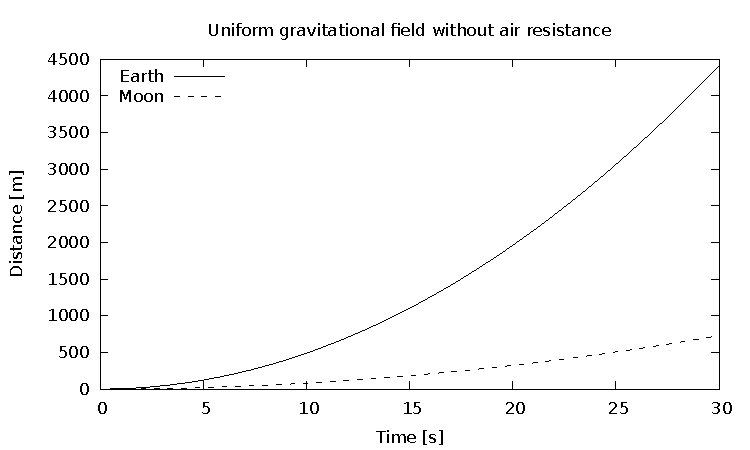
\includegraphics{gnuplot-bw}
% 	\caption{Černobílá varianta obrázku generovaného programem Gnuplot}\label{fig:gnuplot-bw}
% \end{figure}
% 
% \begin{figure}\centering
% 	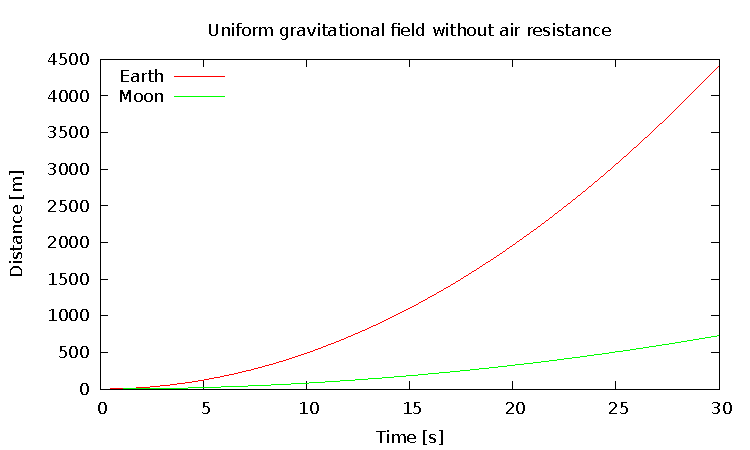
\includegraphics{gnuplot-col}
% 	\caption{Barevná varianta obrázku generovaného programem Gnuplot}\label{fig:gnuplot-col}
% \end{figure}
% 
% 
% \subsection{Tabulky}
% 
% Tabulky lze zadávat různě, např. v~prostředí \verb|tabular|, avšak pro jejich vkládání platí to samé, co pro obrázky -- použijte plovoucí prostředí, v~tomto případě \verb|table|. Například tabulka \ref{tab:matematika} byla vložena tímto způsobem.
% 
% \begin{table}\centering
% 	\caption[Příklad tabulky]{Zadávání matematiky}\label{tab:matematika}
% 	\begin{tabular}{|l|l|c|c|}\hline
% 		Typ		& Prostředí		& \LaTeX{}ovská zkratka	& \TeX{}ovská zkratka	\tabularnewline \hline \hline
% 		Text		& \verb|math|		& \verb|\(...\)|	& \verb|$...$|		\tabularnewline \hline
% 		Displayed	& \verb|displaymath|	& \verb|\[...\]|	& \verb|$$...$$|	\tabularnewline \hline
% 	\end{tabular}
% \end{table}
% 
% % % % % % % % % % % % % % % % % % % % % % % % % % % % 

% \chapter{Obsah přiloženého CD}

% %upravte podle skutecnosti

% \begin{figure}
% 	\dirtree{%
% 		.1 readme.txt\DTcomment{stručný popis obsahu CD}.
% 		.1 exe\DTcomment{adresář se spustitelnou formou implementace}.
% 		.1 src.
% 		.2 impl\DTcomment{zdrojové kódy implementace}.
% 		.2 thesis\DTcomment{zdrojová forma práce ve formátu \LaTeX{}}.
% 		.1 text\DTcomment{text práce}.
% 		.2 thesis.pdf\DTcomment{text práce ve formátu PDF}.
% 		.2 thesis.ps\DTcomment{text práce ve formátu PS}.
% 	}
% \end{figure}

\end{document}
